\documentclass{article}
\usepackage[T2A]{fontenc} 
\usepackage[utf8]{inputenc} 
\usepackage[english,russian]{babel}
\usepackage{graphicx} 
\usepackage{amsmath}
\usepackage{amsfonts} 
\usepackage{titlesec}
\usepackage{listings}
\usepackage{float}
\usepackage{longtable}
\usepackage{titling} 
\usepackage{geometry} 
\usepackage{pgfplots}
\pgfplotsset{compat=1.9}
\usepackage{xcolor}
\definecolor{darkgreen}{RGB}{0,100,0}

\lstset{
  language=Python,
  basicstyle=\ttfamily,
  keywordstyle=\color{darkgreen},
  stringstyle=\color{purple},
  commentstyle=\color{green},
  morecomment=[l][\color{magenta}]{\#},
  frame=single, 
  showspaces=false, 
  showstringspaces=false, 
  numbers=left, 
  numberstyle=\tiny,
}

\titleformat{\section}
  {\normalfont\Large\bfseries}{\thesection}{1em}{}
\titleformat{\subsection}
  {\normalfont\large\bfseries}{\thesubsection}{1em}{}

\setlength{\droptitle}{-6em} 
\title{Отчет по лабораторной работе № 4\\ Вариант № 3}
\author{Винницкая Дина Сергеевна}
\date{Группа: Б9122-02-03-01сцт}

\geometry{a4paper, margin=2cm}

\begin{document}

\maketitle
\section*{Цель работы}
\begin{enumerate}
    \item $\text{Вычислить интеграл:} \quad \int_{a}^{b} f(x)dx \quad \text{по составной формуле центральных прямоугольников}; $
    \item  Получить формулу для численого интегрирования методом центральных прямоугольников в виде $ I = \displaystyle\sum_{i=0}^{n} c_i \cdot f(x_i);$
    \item Исследовать порядок аппроксимации метода. Получить теоретическую оценку для $R_n$
    \item Провести вычислительный эксперимент для $n = \{2, 4, 8, 16,…, 2^15\} $
    \item  Сделать ввод о поведении ошибки;
    \item Сделать сравнительную характеристику изветсных методов, таких как методов прямоугольников, трапеций, формулы Симпсона для n = 10000;
    \item На основе полученных данных сделать вывод о эффективности метода центральных прямоугольников;
    \item Заключение.

    
\end{enumerate}

\section*{Входные данные:}
\begin{enumerate}

    \item \textbf{Функция:} $y=x^2 + \ln(x) - 4$
    \item \textbf{Отрезок} $[ 1.5,2.0 ]$

\end{enumerate}

\section*{$\text{Вычисление интеграла:} \quad \int_{a}^{b} f(x)dx $}
Подставим известные значения $\textbf{a}$, $\textbf{b}$ и функцию. Получим:
$$\int_{1.5}^{2} (x^2 + \ln(x) - 4) dx = \int x^2 dx  + \int \ln{x} dx - \int 4 dx = (\frac{x^3}{3} + \ln{n} \cdot x - 5x)\Big|_{1.5}^{2} = \frac{2^3}{3} + \ln{2} \cdot 2 - 5 \cdot 2 - \left(\frac{1.5^3}{3} + \ln{1.5} \cdot 1.5 - 5 \cdot 1.5 \right) =  $$
$$= -\frac{23}{24} + \ln{\frac{8\sqrt{6}}{9}} \approx -0.180237 $$


\section*{Получение формулу  $ I = \displaystyle\sum_{i=0}^{n} c_i \cdot f(x_i);$}
$$ \displaystyle\sum_{i=0}^{n - 1} f(x_{i + \frac{1}{2}}) \int_{x_i}^{x_i + 1} \frac{x - x_i}{x_{i + \frac{1}{2}} - x_i} dx =  \displaystyle\sum_{i=0}^{n - 1} f(x_{i + \frac{1}{2}}) \int_{x_i}^{x_i + 1} \frac{2 (x - x_i)}{h} dx  =\displaystyle\sum_{i=0}^{n - 1}  f(x_{i + \frac{1}{2}}) \cdot \frac{1}{h} (x_{i + 1} - x_i )^2 = \displaystyle\sum_{i=0}^{n - 1} f(x_{i + \frac{1}{2}}) \cdot h$$

\section*{Определение порядка аппроксимации:}

$$R_n(x) = \int_{a}^{b} f(x) \, dx - \sum_{i=0}^{n} f(x_{i + \frac{1}{2}})\cdot h = \int_{a}^{b} f(x) dx -  \sum_{i=0}^{n} f(x_{i + \frac{1}{2}}) (x_i - x_{i - 1}) = $$
$$ = \int_{a}^{b} f(x) dx -  \sum_{i=0}^{n} \int_{x_{i - 1}}^{x_i} f(x_{i - \frac{1}{2}}) dx =  \sum_{i=0}^{n} \int_{x_{i - 1}}^{x_i} f(x_{i - \frac{1}{2}}) dx $$
$$ \sum_{i=0}^{n} \int_{x_{i - 1}}^{x_i} \left(f(x_{i - \frac{1}{2}}) + f`(x_{i - \frac{1}{2}) \cdot (x - x_{i - \frac{1}{2}}}) + \frac{f``(x_{i - \frac{1}{2}})}{2} \cdot (x - x_{i - \frac{1}{2}})^2  \right) = $$
$$ = \sum_{i=0}^{n} \left( \frac{f`(x_{i - \frac{1}{2}})}{2} \left((x_{i + 1} - x_{i - \frac{1}{2}})^2 - (x_i - x_{i - \frac{1}{2}})^2 \right) + \frac{f``(x_{i - \frac{1}{2}})}{6} \cdot \left((x_{i + 1} - x_{i - \frac{1}{2}})^3 - (x_{i} - x_{i - \frac{1}{2}})^3 \right)\right) = $$
$$\sum_{i=0}^{n} \frac{f``(x_{i - \frac{1}{2}})}{2} \cdot \left( \left(\frac{h}{2} \right)^3 - \left(-\frac{h}{2} \right)^3 \right) = \sum_{i=0}^{n} \frac{f``(x_{i - \frac{1}{2}})}{6} \cdot \left(\frac{h^3}{8} + \frac{h^3}{8} \right) \leq \frac{M}{24} \cdot (b - a) \cdot h^2 $$
$$ \sup\limits_{a \leq x \leq b} |f''(x)| = M $$
Из этого можно сделать вывод о том, что $\textbf{порядок аппроксимации второй}.$
\section*{Реализация алгоритма:}
\textbf{\large{Опредение основных функций}}

\begin{lstlisting}
def func(x):
    return x ** 2 + sp.log(x) - 4
\end{lstlisting}


\begin{lstlisting}
def f_derivative(x, k):
    if k == 1:
        return 2 * x + 1 / x
    elif k == 2:
        return 2 - 1 / x ** 2
    return (-1) ** ((k % 2) + 1) * factorial(k - 1) / x ** k
\end{lstlisting}

\begin{itemize}
\item Функция \textbf{ f\_derivative(x, k)} Это функция, которая вычисляет производную k-того порядка функции f(x) в точке x. Она предоставляет возможность вычисления производной желаемой степени k в точке x.
\end{itemize}

\begin{lstlisting}
def middle_rectangular(func, a, b, n):
    h = (b - a) / n
    return sum(func(a + h * (i + 0.5)) * h for i in range(n))
\end{lstlisting}

\begin{itemize}
\item Функция \textbf{middle\_rectangular(func, a, b, n)} Используя метод центральных прямоугольников, эта функция вычисляет аппроксимацию интеграла функции func на интервале от a до b с использованием n прямоугольников.
\end{itemize}



\begin{lstlisting}
def mr_error(func, a, b, n):
    m = max(abs(f_derivative(a + (b - a) 
    * i / 1000, 2)) for i in range(1001))
    return m / 24 * (b - a) ** 3 / n ** 2
\end{lstlisting}


\begin{itemize}
\item Функция \textbf{mr\_error(func, a, b, n)} Эта функция вычисляет теоретическую оценку погрешности для метода центральных прямоугольников, используемую для оценки точности аппроксимации интеграла.
\end{itemize}


\begin{lstlisting}
def left_rectangular(func, a, b, n):
    h = (b - a) / n
    return sum(func(a + h * i) * h
               for i in range(n))
\end{lstlisting}

\begin{itemize}
\item Функция \textbf{left\_rectangular(func, a, b, n)} Эта функция вычисляет аппроксимацию интеграла функции func на интервале от a до b с использованием n прямоугольников, используя левые прямоугольники.
\end{itemize}

\begin{lstlisting}
def right_rectangular(func, a, b, n):
    h = (b - a) / n
    return sum(func(a + h * i)
               for i in range(1, n + 1)) * h
\end{lstlisting}

\begin{itemize}
\item Функция \textbf{right\_rectangular(func, a, b, n)} Эта функция вычисляет аппроксимацию интеграла функции func на интервале от a до b с использованием n прямоугольников, используя правые прямоугольники.
\end{itemize}

\begin{lstlisting}
def trapezoidal(func, a, b, n):
    h = (b - a) / n
    return ((func(a) + func(b)) / 2 + sum(func(a + h * i)
                    for i in range(1, n))) * h
\end{lstlisting}


\begin{itemize}
\item Функция \textbf{trapezoidal(func, a, b, n)} Эта функция вычисляет аппроксимацию интеграла функции func на интервале от a до b с использованием n трапеций.
\end{itemize}

\begin{lstlisting}
def simpson(func, a, b, n):
    h = (b - a) / n
    return sum(func(a + h * (i - 1)) + 4 * func(a + h * (i - 0.5))
    + func(a + h * (i))
               for i in range(1, n + 1)) * h / 6
\end{lstlisting}

\begin{itemize}
\item Функция \textbf{simpson(func, a, b, n)} Эта функция вычисляет аппроксимацию интеграла функции func на интервале от a до b с использованием n отрезков по формуле Симпсона.
\end{itemize}


\begin{lstlisting}
def l_rect_error(func, a, b, n):
    m = max(abs(f_derivative(a + (b - a) * i / 1000, 1))
    for i in range(1001))
    return m * (b - a) / 2
\end{lstlisting}

\begin{itemize}
\item Функция \textbf{l\_rect\_error(func, a, b, n)} Эта функция вычисляет теоретическую оценку погрешности для метода левых прямоугольников.
\end{itemize}

\begin{lstlisting}
def r_rect_error(func, a, b, n):
    m = max(abs(f_derivative(a + (b - a) * i / 1000, 1)) 
    for i in range(1001))
    return m * (b - a) / 2
\end{lstlisting}

\begin{itemize}
\item Функция \textbf{r\_rect\_error(func, a, b, n)} Эта функция вычисляет теоретическую оценку погрешности для метода правых прямоугольников.
\end{itemize}

\begin{lstlisting}
def trapezoidal_error(func, a, b, n):
    m = max(abs(f_derivative(a + (b - a) * i / 1000, 2)) for i in
    range(1001))
    return m / 12 * (b - a) ** 3 / n ** 2
\end{lstlisting}

\begin{itemize}
\item Функция \textbf{trapezoidal\_error(func, a, b, n)} Эта функция вычисляет теоретическую оценку погрешности для метода трапеций.
\end{itemize}

\begin{lstlisting}
def simpson_error(func, a, b, n):
    m = max(abs(f_derivative(a + (b - a) * i / 1000, 4)) for i in
    range(1001))
    return m / 2880 * (b - a) ** 5 / n ** 4
\end{lstlisting}

\begin{itemize}
\item Функция \textbf{simpson\_error(func, a, b, n)} Эта функция вычисляет теоретическую оценку погрешности для метода Симпсона.
\end{itemize}

\textbf{\large{Составление таблицы значений для метода центральных прямоугольников
}} \\

Для составления таблицы значений для метода центральных прямоугольников необходимо:
\begin{enumerate}
\item Задать начальные значения для интеграла, количество прямоугольников и других параметров.
\item Используя цикл итераций, увеличивать количество прямоугольников, одновременно вычисляя значение интеграла по методу центральных прямоугольников.
\item Рассчитывать абсолютную разницу между точным значением интеграла и вычисленным значением, относительную погрешность и теоретическую погрешность метода.

\end{enumerate}

\begin{lstlisting}
result = {'j': [], 'n': [], 'I_n': [], 'delta_I_n': [], 'relative_I_n': [],
          'R_n': [], 'growth': [0]}
for i in range(15):
    n *= 2
    I_n = middle_rectangular(func, a, b, n)
    result['j'].append(i + 1)
    result['n'].append(n)
    result['I_n'].append(I_n)
    result['delta_I_n'].append(abs(I - I_n))
    result['relative_I_n'].append(result['delta_I_n'][i] / abs(I) * 100)
    result['R_n'].append(mr_error(func, a, b, n))
    if i > 0:
        result['growth'].append(result['delta_I_n'][i] /
        result['delta_I_n'][i - 1])

df_middle_rect = pd.DataFrame({
    'Iteration': result['j'],
    'n': result['n'],
    'I_n': result['I_n'],
    'Delta I_n': result['delta_I_n'],
    'Relative Error (%)': result['relative_I_n'],
    'R_n': result['R_n'],
    'Growth': result['growth']
})

print(df_middle_rect)
\end{lstlisting}

В результате получим таблицу:
\begin{figure}[h]
    \centering
    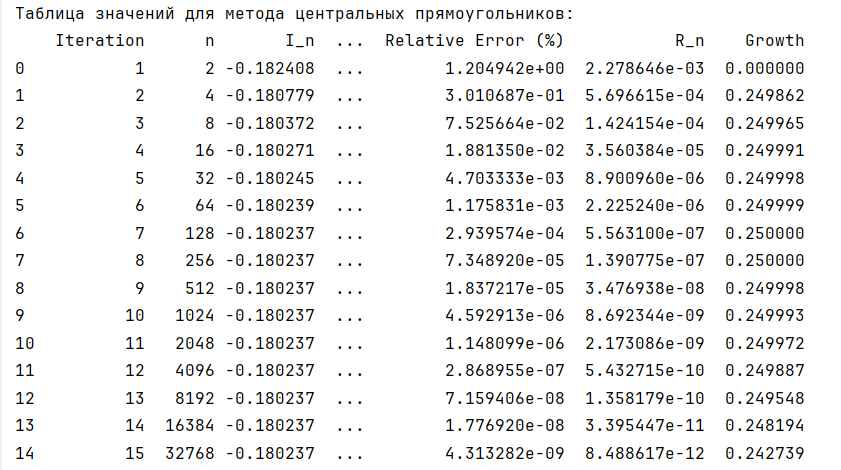
\includegraphics[width=1\textwidth]{lab_4_1.png}
    \caption{ Таблица значений для метода центральных прямоугольников}
    \label{fig:my_label}
\end{figure}


\textbf{\large{Ввод о поведении ошибки}} \\

\begin{itemize}
    \item Исходя из табличных значений абсолютная ошибка близка по значению с теоретической, но по значению, все же незначительно меньше последней. Изменение абсолютной ошибки примерно соответствует увеличению $n$ в степени порядка аппроксимации. Таким образом, с $j=1$ до $j=7$ изменение ошибки разительно увеличивается, то есть абсолютная ошибка незначительно уменьшается. На $j=7$, $j=8$ достигает максимального значения 0.25, а затем начинает уменьшаться до $j=15$.
\end{itemize}

\textbf{\large{Составление сравнительной таблицы различных методов численного интегрирования.}} \\

Для получения сравнительной таблицы различных методов численного интегрирования можно использовать следующий математический алгоритм действий

\begin{enumerate}
\item Для каждого из пяти методов численного интегрирования (левых, правых и центральных прямоугольников, метода трапеций и метода Симпсона) задаются соответствующие функции и оценки погрешности.
\item Циклом происходит вычисление значений интегралов и оценок погрешности для каждого метода.
\item Собираются данные о значениях интегралов, абсолютных различиях, относительных погрешностях и теоретических погрешностях для каждого метода в таблицу.

\end{enumerate}


\begin{lstlisting}
calculate = {'method': ['Left Rectangular', "Right Rectangular",
"Midpoint Rectangular", "Trapezoidal", "Simpson"],
            'I_n': [], 'delta_I_n': [], 'relative_I_n': [], 'R_n': []}
for i, (formula, error) in enumerate([(left_rectangular, l_rect_error), 
(right_rectangular, r_rect_error),
                                     (middle_rectangular, mr_error), 
                                     (trapezoidal, trapezoidal_error),
                                     (simpson, simpson_error)]):
   calculate['I_n'].append(formula(func, a, b, 10000))
   calculate['delta_I_n'].append(abs(I - calculate['I_n'][i]))
   calculate['relative_I_n'].append(calculate['delta_I_n'][i] / abs(I) * 100)
   calculate['R_n'].append(error(func, a, b, 10000))

table_headers = ['Method', 'I_n', 'delta_I_n', 'relative_I_n', 'R_n']
table_data = [["Left Rectangular", calculate['I_n'][0], 
    calculate['delta_I_n'][0], calculate['relative_I_n'][0],
              calculate['R_n'][0]],
             ["Right Rectangular", calculate['I_n'][1],
             calculate['delta_I_n'][1], calculate['relative_I_n'][1],
              calculate['R_n'][1]],
             ["Midpoint Rectangular", calculate['I_n'][2], 
             calculate['delta_I_n'][2],
              calculate['relative_I_n'][2],
              calculate['R_n'][2]],
             ["Trapezoidal", calculate['I_n'][3], calculate['delta_I_n'][3],
             calculate['relative_I_n'][3],
              calculate['R_n'][3]],
             ["Simpson", calculate['I_n'][4], calculate['delta_I_n'][4], 
             calculate['relative_I_n'][4],
              calculate['R_n'][4]]]

print(tabulate(table_data, headers=table_headers, tablefmt='grid'))

\end{lstlisting}

В результате получим таблицу:
\begin{figure}[H]
    \centering
    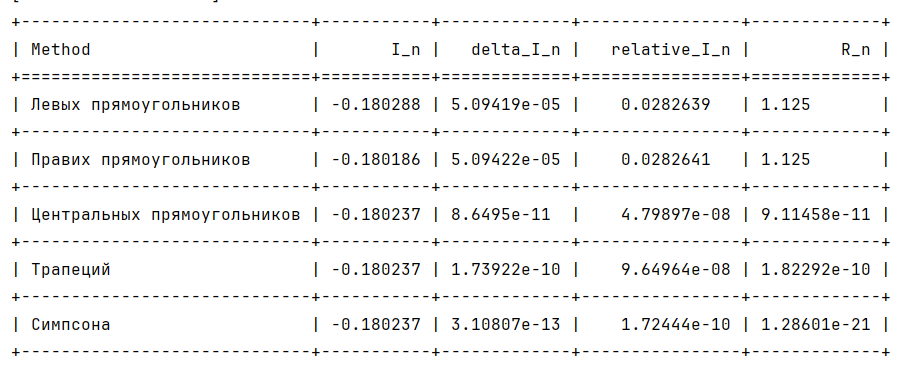
\includegraphics[width=1\textwidth]{lab_4_2.png}
    \caption{ Сравнительная таблица различных методов численного интегрирования}
    \label{fig:my_label}
\end{figure}


\textbf{\large{Вывод о эффективности метода центральных прямоугольников}} \\
\begin{itemize}
    \item В данном случае метод центральных прямоугольников продемонстрировал второй по эффективности результат среди рассмотренных методов численного интегрирования (с учетом абсолютной, относительной и теоретической погрешностей). Он выдал более точные значения, чем методы левых и правых прямоугольников, а также метод трапеций, однако оказался значительно менее точным, чем метод Симпсона, как и все остальные перечисленные методы.
\end{itemize}

\section*{Заключение}
 \begin{itemize}
     \item В ходе выполнения лабораторной работы был проведен анализ эффективности различных методов численного интегрирования, таких как левых прямоугольников, правых прямоугольников, центральных прямоугольников, метода трапеций и метода Симпсона.  Результаты показали, что метод центральных прямоугольников оказался крайне эффективным, в сравнении с методами левых и правых прямоугольников, а также методом трапеций. Но, следует заметить, что данный метод значительно уступает методу Симпсона, который продемонстрировал наилучшие результаты.
     \item Полученные данные позволяют сделать вывод о том, что выбор метода численного интегрирования зависит от требуемой точности и эффективности.
     \item Также в ходе лабораторной работы были получены таблицы  значений для метода центральных прямоугольников и сравнения различных методов численного интегрирования, благодаря которым и был аргументирован полученный вывод.
     
 \end{itemize}

 \textbf{\large{Ниже будут продублированы результирующие таблицы}} \\
 

 \begin{table}[H]
\centering
\begin{tabular}{|c|c|c|c|c|c|c|}
\hline
i & n & $I_n$ & $\Delta I_n$ & $\delta I_n$ & R_n & $\frac{\Delta I_{2^j}}{\Delta I_{2^{j - 1}}}$ \\
\hline
1 & 2 & -0.182408 & 2.171747e-03  & 1.204942e+00 & 2.278646e-03 & 0.000000 \\
2 & 4 & -0.180779 & 5.426361e-04 & 3.010687e-01 & 5.696615e-04 & 0.249862 \\
3 & 8 & -0.180372 & 1.356400e-04  & 7.525664e-02 & 1.424154e-04 & 0.249965 \\
4 & 16 & -0.180271 & 3.390882e-05  & 1.881350e-02 & 3.560384e-05 & 0.249991 \\
5 & 32 & -0.180245 & 8.477130e-06  & 4.703333e-03 & 8.900960e-06 & 0.249998 \\
6 & 64 & -0.180239 & 2.119277e-06  & 1.175831e-03 & 2.225240e-06 & 0.249999 \\
7 & 128 & -0.180237 & 5.298189e-07  & 2.939574e-04 & 5.563100e-07 & 0.250000 \\
8 & 256 & -0.180237 & 1.324545e-07 & 7.348920e-05 & 1.390775e-07 & 0.250000 \\
9 & 512 & -0.180237 & 3.311338e-08 & 1.837217e-05 & 3.476938e-08 & 0.249998 \\
10 & 1024 & -0.180237 & 8.278112e-09  & 4.592913e-06 & 8.692344e-09 & 0.249993 \\
11 & 2048 & -0.180237 & 2.069295e-09  & 1.148099e-06 & 2.173086e-09 & 0.249972 \\
12 & 4096 & -0.180237 & 5.170908e-10  & 2.868955e-07 & 5.432715e-10 & 0.249887 \\
13 & 8192 & -0.180237 & 1.290387e-10 & 7.159406e-08 & 1.358179e-10 & 0.249548 \\
14 & 16384 & -0.180237 & 3.202660e-11  & 1.776920e-08 & 3.395447e-11 & 0.248194 \\
15 & 32768 & -0.180237 & 7.774115e-12 & 4.313282e-09 & 8.488617e-12 & 0.242739 \\
\hline
\end{tabular}
\caption{Таблица значений для метода центральных прямоугольников}
\label{tab:my_label}
\end{table}


\begin{table}[H]
\centering
\begin{tabular}{|c|c|c|c|c|}
\hline
Method & $I_n$ & delta$I_n$ & Relative$I_n$ & $R_n$ \\
\hline
Левых
прямоугольников& -0.180288 & 5.09419e-05 & 0.0282639 & 1.125 \\
Правих
прямоугольников & -0.180186 & 5.09422e-05 & 0.0282641 & 1.125 \\
Центральных
прямоугольников & -0.180237 & 8.6495e-11 & 4.79897e-08 & 9.11458e-11 \\
Трапеций  & -0.180237 & 1.73922e-10 & 9.64964e-08 & 1.82292e-10 \\
Симпсона  & -0.180237 & 3.10807e-13 & 1.72444e-10 & 1.28601e-21 \\
\hline
\end{tabular}
\caption{Сравнительная таблица различных методов численного интегрирования}
\label{tab:my_label_2}
\end{table}


\end{document}

